

\section*{{Abstract:}}


	Many cities have undergone spatial re-distributions of low-income populations from central to suburban neighborhoods over the past several decades. A potential negative impact of these trends is that low-income populations are concentrating in more automobile oriented areas and thus resulting in increased barriers to daily travel and activity participation, particularly for those who are unable to afford a private vehicle. Accordingly, the objective of this paper is to analyze the links between increasing socio-spatial inequalities, transport disadvantage, and adverse travel behaviour outcomes. This is examined first from a theoretical perspective, and second via a spatio-temporal analysis for the Toronto region from 1991 to 2016. Findings show that many suburban areas in Toronto are not only declining in socioeconomic status, but are also suffering from increased barriers to daily travel evidenced by longer commute times and decreasing activity participation rates, relative to central neighborhoods. Because of these adverse effects, this evidence further supports the need for progressive planning and policy aimed at curbing continuing trends of suburbanization of poverty while also improving levels of transport accessibility in the suburbs.



\section*{{Keywords:}}

transportation, neighborhood change, poverty, daily travel, suburbs








\normalsize




\section{Introduction}

% background
In most early industrializing cities, poverty was traditionally clustered within central areas, while the more affluent lived in peripheral parts of cities away from heavy industry and pollution. During the mid-20th century, many cities have de-industrialized, resulting in increased demand for inner-city living and investment in housing stock in central areas. One effect of this in some cities is that the costs of housing in central areas has increased substantially, causing the spatial distribution of lower-income households to shift to less central, but more affordable, peripheral neighborhoods \shortcite{kneebone_suburbanization_2010,ehrenhalt_great_2012,howell_racial_2014,pavlic_declining_2014,cooke_suburbanization_2015,ades_is_2016}. 

% problem
A potential negative impact of these trends is that low-income households are re-locating to areas that are more auto-oriented, less walkable, and have relatively lower levels of public transit service than central areas. This could be resulting in longer commutes and increased barriers to daily activity participation, especially for those who are unable to afford a private vehicle. The ability to travel to important activity destinations is vital for economic independence (e.g. finding and retaining employment), health, and well-being - and at a greater scale, it can contribute to robust urban economies and healthier societies as a whole. In the worst cases, dissuasion or inability to travel to important destinations can limit activity participation, result in social exclusion, and negatively impact the vitality of urban environments \cite{lucas_transport_2012,martens_transport_2016}.

% research goal and methods
Accordingly, the objective of this paper is to describe the links between increasing socio-spatial inequalities (e.g. de-centralization of low-income households), transport disadvantage (e.g. spatial distribution of zero-car households, low levels of transit accessibility), and adverse travel behaviour outcomes (e.g. lengthier commute times and lower activity participation rates). This is discussed first from a theoretical standpoint with reference to existing research, then a neighborhood level empirical investigation is conducted for the Toronto region, a city that is experiencing growing income inequalities and concentrations of poverty in more suburban areas \shortcite<e.g.>{hulchanski_three_2010,walks_social_2001,ades_are_2012,breau_pulling_2018}.
This exploratory investigation is informed through six periods of the quinquennial Canadian census and a regional travel survey (from 1991 to 2016) in order to describe neighborhood-level changes in socio-economic status (SES) \textit{vis-\`a-vis} changes in transport disadvantage and travel behaviour outcomes. Our methods include computing transit accessibility metrics that are comparable over time, statistical mapping, modelling changes in travel behaviour over time, and visualizing neighborhood change with respect to levels of suburbanization. While focused on Toronto, these methods can be transferable to other regions.

% key results 
The key finding of our analysis is that social and transport disadvantage are increasing more in the suburbs relative to central areas, leading to adverse travel behaviour outcomes such as increasing commute times and lowering activity participation rates. Policy and planning strategies to reduce these negative outcomes should thus focus both on curbing trends of suburbanization of poverty as well as reducing levels of transport disadvantage in suburban neighborhoods. 




\section{Background}


Suburbanization of poverty refers to the spatial re-distributions of low-SES households from central to suburban neighborhoods, usually in reference to changes occurring during the latter half of the 20th century and early 21st century. Recent research has highlighted trends of suburbanization of poverty in early-industrializing cities in nations such as the United States
\cite{kneebone_suburbanization_2010,howell_racial_2014,cooke_suburbanization_2015}, the Netherlands \cite{hochstenbach_gentrification_2018}, Sweden \shortcite{hedin_neoliberalization_2012}, Scotland \cite{kavanagh_is_2016}, and Australia \cite{randolph_suburbanizing_2014}.
% From a research perspective, empirical evidence on suburbanization of poverty is usually based on longitudinal analysis of census data or specific panel surveys analyzing changes in the spatial distribution of low-income households or other SES variables over time.

% Canada
In Canada, there is evidence of increasing income inequalities both within and between regions
\cite{walks_income_2013,bolton_growing_2012,breau_rising_2015,chen_why_2012}, 
% maclachlan_measures_1997
as well as concentrations of low-income households forming in some inner-suburban neighborhoods
\cite{ades_are_2012,pavlic_declining_2014,ades_is_2016,breau_pulling_2018}.
For example, \citeA{pavlic_declining_2014} classified census tracts by density, age of housing stock, and distance to downtown and found that there has been decline or stagnation in prosperity in inner-suburban areas relative to central areas and newer outer-ring suburbs. Research by \shortciteA{ross_dimensions_2004} and \shortciteA{ades_are_2012} computed spatial segregation indices on low-income households and households in poverty in Canadian cities, each finding that economic segregation is increasing at a neighborhood level and that low-income households are becoming increasingly concentrated and isolated within cities' spatial units. Statistical mapping exercises have also highlighted that neighborhoods with higher concentrations of low-income households are located further from the downtown core over the past several decades \cite{ades_are_2012,breau_pulling_2018}.


% concerns
These trends of suburbanization of poverty have raised concerns regarding the increasing polarization and segregation of urban space by class and income \cite{hulchanski_three_2010,walks_income_2013,ades_are_2012}, as well as negative impacts caused by eviction and displacement on individual well-being and disrupted community cohesion \cite{august_challenging_2014,august_its_2016}. There are also increasing concerns that low-income households now have greater levels of transport disadvantage than in previous decades due to being located further from major employment centres and living in neighborhoods with less walkable environments and lower levels transit service, limiting their ability to travel to and participate in daily activities, particularly for those who are unable to afford a private car \cite{skaburskis_filtering_2014,ades_are_2012}. However, the transport-related impacts of suburbanization of poverty remain largely understudied.



% \section{Transport Poverty}

%- overview
A primary goal of urban transport is to provide people the ability to travel to daily activities in a reasonable amount of time \cite{martens_transport_2016}. If people are not able to do so it indicates that the transportation network is not fulfilling its intended purpose. Travel costs are generally felt to a greater degree by lower-income households (e.g. owning or leasing a private car is a luxury that many lower-income households cannot afford). Transport disadvantage (e.g. such as not having access to a car, living in a neighbourhood with low levels of public transit service, etc.) can admix with other forms of social disadvantage (e.g. unemployment, low income, etc.) resulting in negative outcomes like lengthy commutes and barriers to participating in daily activities \shortcite{lucas_transport_2012,lucas_is_2018}. This combined effect is often called transport poverty. This is more likely to occur for lower-SES residents who live in suburban environments as these environments typically have lower levels of transit service and often require the use of private cars, which for many low-income households, are not affordable.

% evidence on transport poverty
Several research projects have empirically analyzed how transport disadvantage can negatively impact activity participation for more at-risk groups like low-income households \shortcite<e.g.>{farber_my_2009,roorda_trip_2010,lucas_modelling_2016,allen_planning_2020}. % casas_social_2007
Auto-oriented environments can also dissuade active transportation like walking or cycling, for example, due to limited or unsafe pedestrian and cycling infrastructure or simply because destinations are too far away \cite{cervero_travel_1997,ewing_travel_2010}. 
While some low-income households that live in suburban environments may be able to afford a car, they are often at greater risk of going into debt because of needing high-interest loans \cite{walks_driving_2018}, being more susceptible to feeling the effects of rising fuel costs \shortcite{mattioli_vulnerability_2019},
% mattioli_vulnerability_2018
and are more likely to drive cars that are used and unreliable, and therefore riskier purchases, despite their lower upfront costs \cite{klein_desperately_2020}. These financial costs of private car access for lower-income households can increase financial stress and cause households to limit spending on other important areas (e.g. housing, healthy food, etc.).

% existing work on estiming where it's a problem - scale, etc.
Accordingly, there have been several recent studies that have analyzed how and where transport disadvantage aligns with socio-economic groups who are more vulnerable to experiencing transport poverty, both in Canada \cite<e.g.>{foth_towards_2013,allen_sizing_2019} and elsewhere \cite<e.g.>{currie_quantifying_2010,fan_impact_2012,dejohn_transit_2019}. 
These studies have either looked at the overall equity of transit systems, for example analyzing whether transit is adequately serving low-SES areas relative to other areas, or have focused on highlighting areas that have high risk of transport poverty; neighborhoods where low-SES households have inadequate public transit service. Generally, transit service is found to be equitable in most cities in the sense that transit is serving neighborhoods with low-SES households relatively more than overall populations. This is unsurprising since lower-income households live in smaller units with higher levels of population density and are more likely to want to live in areas with good transit service due to lack of car ownership. Also, more affluent households generally have less of a preference to live near transit due to being able to afford a car \cite{glaeser_why_2008}.

% discussion with links with sub poverty / neighborhood change
However, given existing trends of suburbanization of poverty, there are now more low-income households in suburban areas than in previous decades in many cities \cite{ades_are_2012,ades_is_2016,breau_pulling_2018}. This is potentially increasing the risks of transport poverty, and further exasperating urban inequalities more generally. However, it remains unknown how the risks of transport poverty are increasing in cities alongside trends of suburbanization of poverty. Research on neighborhood socio-economic change has typically not included transport variables like transit accessibility, car ownership, commute times, and activity participation rates - key indicators of transport poverty and its outcomes. There have been a few studies that descriptively examine changes in public transit accessibility over time alongside changes in neighborhood level socio-economic status \shortcite{foth_towards_2013,farber_transit_2017,deboosere_understanding_2019}. However, these have been predominantly focused on public transit infrastructure, and did not consider car-ownership, an important component of transport (dis)advantage, nor have they considered outcomes such as activity participation. They are also only focused on a short time period or only consider the impacts of specific transit lines, rather than examining region wide changes over periods longer than a decade. There is some research by transportation engineers on analyzing changes in trip and activity rates over longer periods time \shortcite<e.g.>{roorda_two_2008,kasraian_multi-decade_2020,ozonder_longitudinal_2020}. 
% kitamura_formulation_1988, % miller_evolution_2003
These studies tend to focus on aggregate trends at a regional level or improving the predictive capability of travel demand models, but they provide little insight on the links between travel behaviour with neighborhood-level demographic changes, increasing income inequalities, and geographies of transport disadvantage. Accordingly, the goal of the following analysis is to develop deeper understanding of where and to what extent suburbanization of poverty is potentially increasing the risks of barriers to daily travel, in order to better inform policy and planning aimed at reducing these risks. 





\section{Study Area and Data}

The study area for this paper is the Toronto Census Metropolitan Area (CMA). CMAs are agglomerations of municipalities where at least 50\% of the labour force works within the region's core. While not a perfect definition of what counts as an urban region, it is consistent with what has been used in previous research on the Toronto area regarding neighborhood change, socio-spatial polarization, and suburbanization of poverty \shortcite<e.g.>{walks_social_2001,ross_dimensions_2004,ades_are_2012,ades_is_2016}. 
Table \ref{table:summary} indicates how the region has grown from 1991 to 2016, both in terms of population and built-up area.


\begin{table}[h]
	\small
	
	\caption{{Summary statistics of the Toronto CMA from 1991 to 2016}}
	\label{table:summary}
	\begin{adjustwidth}{-1in}{-1in}
		\centering
	\begin{tabular}{lcccccc}
		\hline
		\textbf{}                          & \textbf{1991} & \textbf{1996} & \textbf{2001} & \textbf{2006} & \textbf{2011} & \textbf{2016} \\
		\hline
		Population (millions)                      & 3.84   & 4.19   & 4.50   & 5.02   & 5.49   & 5.82   \\
		Dwellings (millions)                       & 1.35   & 1.46   & 1.60   & 1.77   & 1.96   & 2.10   \\
		Jobs (millions)                                                    & 1.87    & 1.96    & 2.22   & 2.28    & 2.50     & 2.60  \\
		Built Up Area (km\textasciicircum{}2)      & 1,700  & 1,900  & 2,100  & 2,200  & 2,200  & 2,300  \\
		
		\hline 
	\end{tabular}
\end{adjustwidth}
\end{table}

\subsection{Data Sources}

Data for this study draws from the long-form Canadian census and the Transportation Tomorrow Survey (TTS), the largest household travel survey in the region. Both of these surveys are conducted quinquennially, within a few months of each other (the census in May and the TTS in September). This allows for them to be analyzed in concordance with little temporal uncertainty. 

The Canadian census is divided into short-form and long-form versions. The short-form only asks questions regarding basic demographic information, while the long-form asks a wider range of questions including, but not limited to, education, housing characteristics, employment, and immigration. The long-form census is administered to 20\% of households in Canada. However, the mandatory long-form census was not conducted in 2011, when it was replaced by the voluntary National Household Survey (NHS). The NHS has been criticized for its geographically varying response rate, which in some cases is correlated with different socio-economic variables. For completeness, we decide to use the NHS data for our analysis, but results for 2011 should be treated with caution and greater uncertainty than other years used in this study.

The TTS is a 5\% sample of households in the Toronto region \cite{ashby_transportation_2016}. Its focus has primarily been on collecting data for regional travel demand models. We use the TTS for variables pertaining to car ownership, commuting behaviour, and activity participation rates. A limitation of this survey and derived data is that it only pertains to a single weekday. As well, like many travel surveys, there are concerns regarding under-reporting due to proxy responses per household, as well as under-reporting of short trips, trips without a specific destination like short recreational trips, or trips undertaken by active modes such as walking and cycling \shortcite{wolf_trip_2003}. Despite these limitations, the TTS is the largest sample travel survey of its kind in Canada, and has been used as the basis for a number of transport planning studies, including longitudinal analyses \shortcite{miller_evolution_2003,roorda_two_2008,kasraian_multi-decade_2020,ozonder_longitudinal_2020}.

Census and TTS data were acquired as aggregate summaries pertaining to neighborhood sized spatial boundaries. TTS data are linked to Traffic Analysis Zones (TAZ) while census data are linked to census tracts. Some of these boundaries were re-delineated over time because of demographic change. To expedite part of our longitudinal analysis, data from each year and each survey are joined to 2016 census tract boundaries via a population-weighted areal interpolation procedure that minimizes error when boundaries change over time (see \citeA{allen_new_2018} for a description of this process). This data harmonization allows for analysis over a 25 year period from 1991 to 2016 at a consistent set of neighborhood-level geographic units ($n$ = 1,133 census tracts)




\subsection{Measuring Social Disadvantage}

Table \ref{table:census} displays the variables from the Canadian census that are used to form our understanding of neighborhood level socio-economic status. This table provides regional context that is important to note prior to examining intra-regional trends. Variables were selected based on two criteria: 1) they have been used in previous studies that have examined social deprivation in Canada \shortcite{pampalon_deprivation_2009} as well as their relation to transport disadvantage \shortcite{foth_towards_2013, el-geneidy_non-stop_2016, allen_sizing_2019}, and 2) variable consistency across multiple census years.

\begin{table}[h]
	\small
	
	\caption{{Summary of Statistics Canada census SES data for the Toronto CMA from 1991 to 2016}}
	\label{table:census}
	\begin{adjustwidth}{-1in}{-1in}
		\centering
	\begin{tabular}{lcccccc}
		\hline
		\textbf{}                          & \textbf{1991} & \textbf{1996} & \textbf{2001} & \textbf{2006} & \textbf{2011} & \textbf{2016} \\
		\hline
		Population (millions)                      & 3.84   & 4.19   & 4.50   & 5.02   & 5.49   & 5.82   \\
		Average household income (in 2016 CAD) & \$92k   & \$87k   & \$100k   & \$104k   & \$102k   & \$112k \\
		\% who live in low-income households                 & 15\% & 21\% & 17\% & 19\% & 15\% & 18\% \\
		\% who have housing cost 30\% or more of their income & 23\% & 37\% & 29\% & 33\% & 32\% & 34\% \\
		\% of dwellings that need major repairs            & 7\%  & 8\%  & 7\%  & 6\%  & 6\%  & 5\%  \\
		
		\% of families that are single-parent families               & 
		14\% & 16\% & 17\% & 17\% & 18\% & 18\% \\
		\% who immigrated internationally in the past 5 years              & 9\%  & 8\%  & 8\%  & 8\%  & 7\%  & 7\%  \\
		\% who do not have a high school diploma    & 33\% & 31\% & 23\% & 20\% & 17\% & 16\% \\
		\% who are unemployed                              & 9\%  & 9\%  & 6\%  & 7\%  & 9\%  & 8\%  \\
		\hline 
	\end{tabular}
\end{adjustwidth}
\end{table}

The regional trends presented in Table \ref{table:census} indicate relative stability in SES over time at an aggregate level, with some exceptions for specific variables. Looking at income, we see that the average income in the region has increased, but there also has been a slight increase in percent of population in low-income households. This deviation aligns with research showing an increase in income polarization in the Toronto region \cite{hulchanski_three_2010}. Education rates have improved substantially in the region over time, from 33\% of adults not having a high school education to only 16\%. Other less pronounced trends over time include relative decreases in dwellings that need major repairs, immigration, and unemployment while there has been a slight increase in percent of single-parent families. Important to note is that relatively stable proportions over time however indicate growing overall counts of people in each group since the overall population of the region is steadily increasing over time (e.g. the total number of people in low income households in 1991 compared to 2016 nearly doubled). The most notable temporal deviation is for 1996, when a recession in the early 1990s explains worse SES indicators for this year (e.g. higher poverty rate, lower average income, greater percent of income devoted to housing).

We also generate a single indicator of neighborhood level socio-economic status using a Principal Components Analysis (PCA) on the variables presented in Table \ref{table:census}. PCAs are commonly used to develop composite indices \cite{oecd_handbook_2008}, including neighborhood-level measures of socio-economic status  \cite{pampalon_deprivation_2009,cabrera-barona_multiscale_2016}. A PCA reduces these correlated observed variables into independent composite variables. Specifically, the results of a PCA are the eigenvectors of the covariance matrix, ranked by how much variance they explain. We considered having more than one indicator of SES, but we found that the first component of the PCA explained 53\% percent of the variance of the eight variables, while the second component only explained 15\% percent. We term this output first principal component as $SES_{i,\gamma}$. It can be represented as a linear combination of the standard score, $Z_{x,i,\gamma}$, of each input variable, $x$, where $i$ pertains to a census tract and $\gamma$ is the year. All variables from all years were normalized prior to the PCA.


\begin{equation}
{SES}_{i,\gamma} = \sum_x w_x Z_{x,i,\gamma} 
\end{equation}

The factor weights, $w_x$, for each variable, $x$, are displayed in Table \ref{table:pca}. Also displayed is the correlation coefficient between $SES_{i,\gamma}$ and $Z_{x,i,\gamma}$. 




The resulting values of $SES_i$ have a mean of zero and a standard deviation equal to two. Also to note is that it has a negative skew ($\bar{\mu}_3$ = -0.75), meaning that wealthier neighborhoods are more similar to each other in terms of SES, while poorer neighborhoods have greater dispersion. This highlights how the poorest neighborhoods are relatively further from the mean that affluent neighbourhoods. Plots of the distribution of $SES_i$ for each year are shown in Figure \ref{fig:SES_violin}. Overall, there is stability in the average levels of SES over time. The notable exception is 1996 where there is a substantial decline in SES, likely due to the early 1990s recession. The relative consistency in distributions of SES by year is contrary to some previous research highlighting increased polarization over time \cite{hulchanski_three_2010}. This is likely because this previous research has focused solely on income inequalities, rather than a composite index of SES. Summary plots like these also mask spatial variations and changes in spatial patterns over time.


\begin{table}[h]
	\small
	\centering
	\caption{{Results of a PCA of neighbourhood level socio-economic status for the Toronto CMA}}
	\label{table:pca}
	\begin{tabular}{lcc}
		
		\hline
		& $w_x$     & corr($SES_{i,\gamma}, Z_{x,i,\gamma}$)   \\
		\hline
		Logged average household income (in 2016 CAD)  & 0.43 & 0.87 \\
		\% who live in low income households     & -0.45  & -0.92  \\
		
		\% who have housing cost 30\% or more of their income & -0.33  & -0.67  \\
		\% of dwellings that need major repairs    & -0.28  & -0.57  \\
		\% of families that are single-parent families     & -0.38  & -0.77  \\
		\% who immigrated internationally in the past 5 years    & -0.30  & -0.62  \\
		\% who do not have a high school diploma  & -0.21  & -0.43  \\
		\% who are unemployed   & -0.39  & -0.79 \\
		\hline
	\end{tabular}
\end{table}



\begin{figure}[H]
	\centering
	
	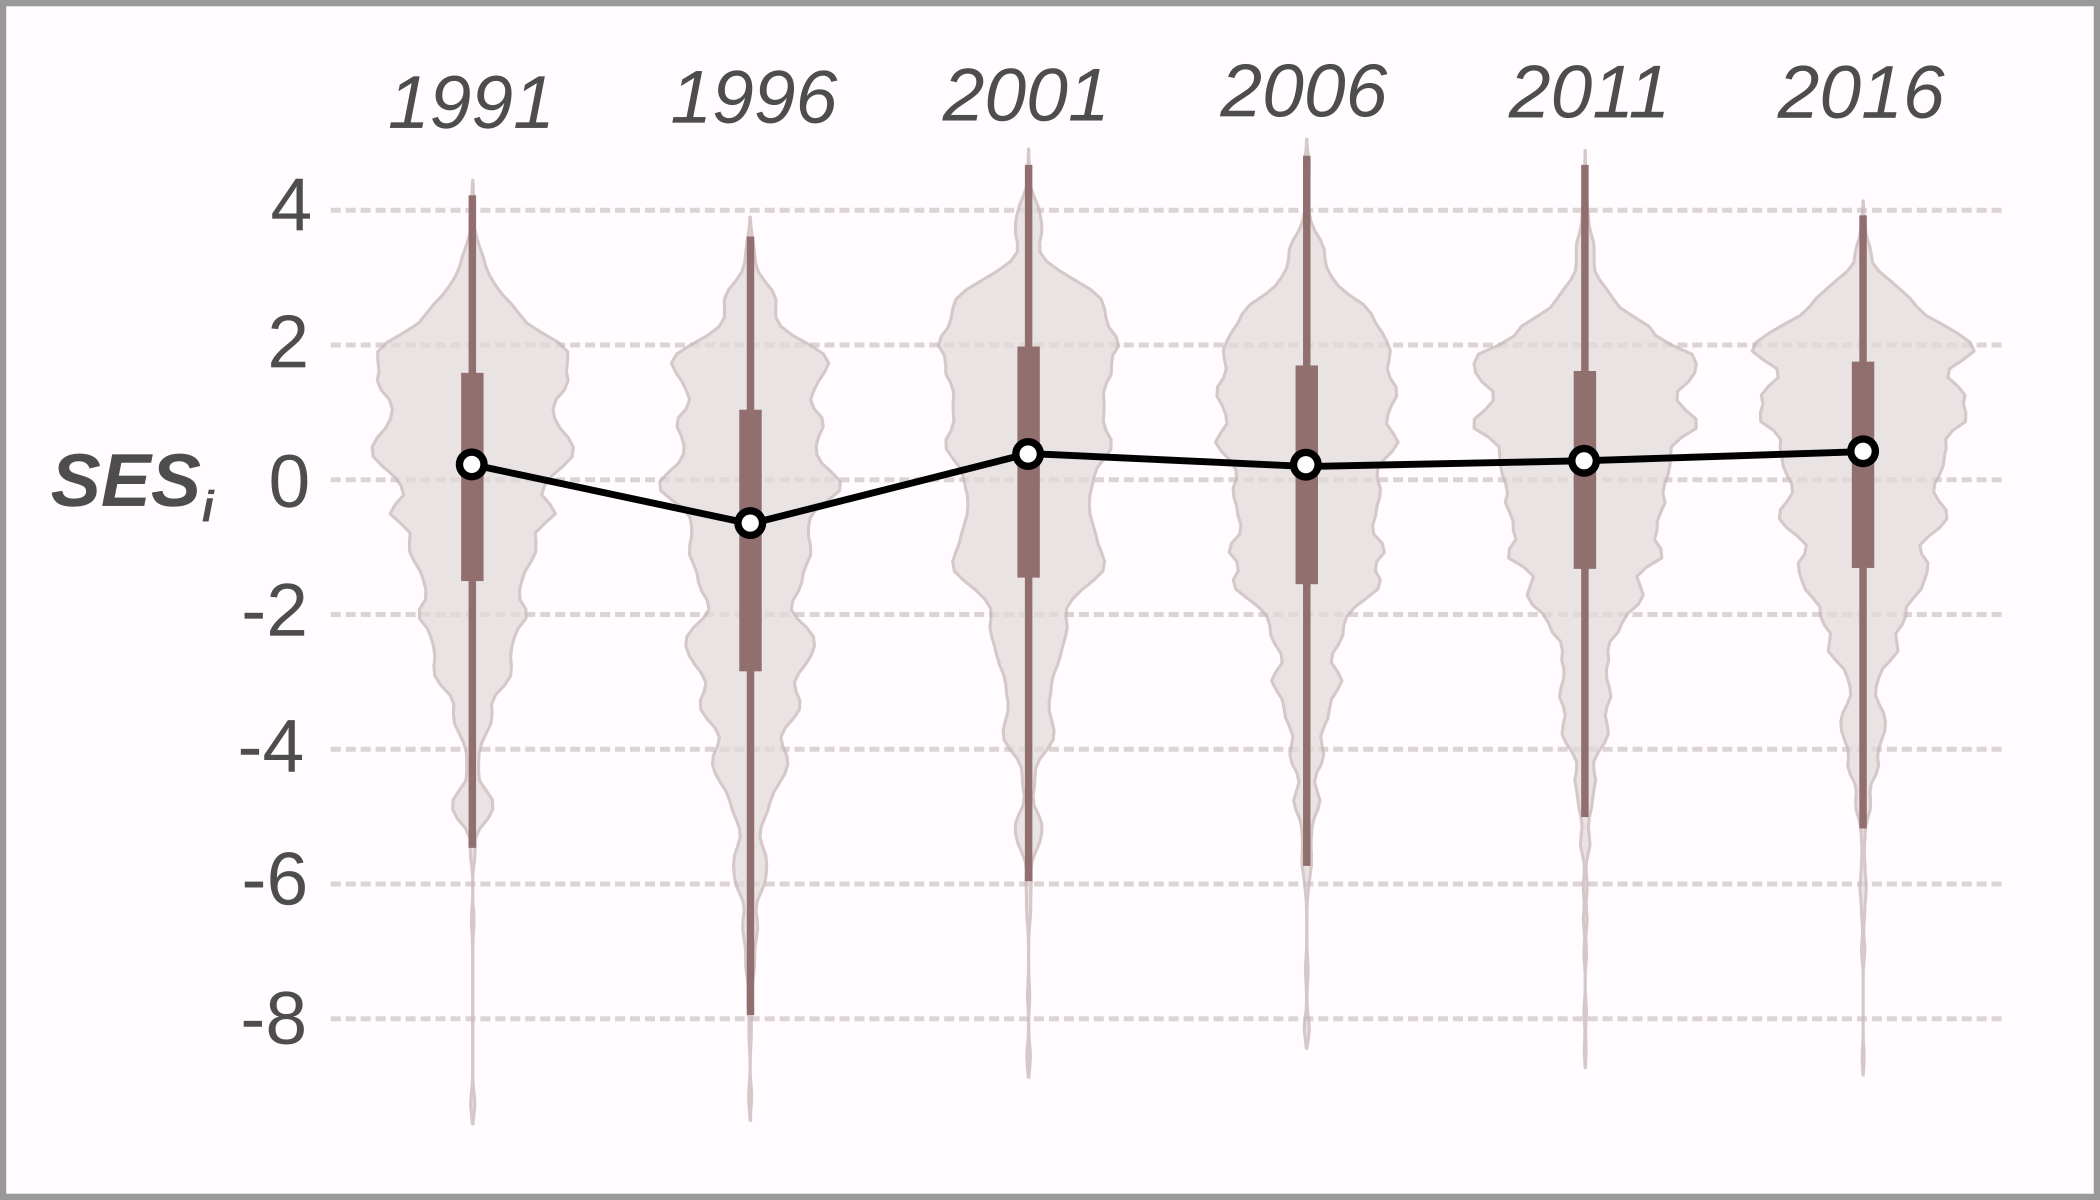
\includegraphics[width=3.5in]{figures/Fig1}
	\caption{{Population weighted distribution in $SES_i$ by year}}
	\label{fig:SES_violin}
	
\end{figure}




\subsection{Measuring Transport Disadvantage}

Transport disadvantage can be considered both in terms of opportunity and outcomes \cite{banister_inequality_2018}. 

For outcomes, we use two travel behaviour variables: activity participation and commute times. Commute times for our analysis are based on historical travel time matrices linked to origin-destination survey data. These travel times were extracted from historical travel demand models of the region for the morning commute period (6:30am to 9:30am) \cite{tmg_gtamodel_2016}. Commute times were averaged by neighborhood. Activity participation is defined as the neighborhood average of the number out-of-home activities people travel to over the course of a day, based on the TTS. At an individual level, the extent of daily activity participation could be a result of preferences or constraints. For example, low levels of activity participation could either be due to not wanting to travel to a destination or due to transport disadvantage (e.g. lack of car access) impeding travel. Moreover, high levels of activity participation may not always be based on choice, but could also be due to the time pressures of working more than one job and balancing household activities. Overall, though, previous research has highlighted how low levels of activity participation predominantly indicates that residents are experiencing barriers to daily travel, and furthermore, has been used as evidence of increased risks of transport-related social exclusion \cite{martens_transport_2016,lucas_is_2018}. For instance, mapping neighbourhood-level "participation deserts" have been used as a transport planning tool to assess which neighbourhoods within are region are suffering the most from transport disadvantage \cite{allen_planning_2020}.  

For opportunity, we consider this in two dimensions as well: transit accessibility and auto availability. For the latter, we compute the percent of households without cars in each neighborhood from the TTS. While it is true that just because a household has a car, it does necessarily mean that it provides an adequate form of mobility for all members of a household (e.g. there may be competition for its use, and the car itself may not be reliable). However, lack of auto availability has been shown to be a substantial barrier for daily travel within North American urban contexts \cite{blumenberg_car-deficit_2018,allen_planning_2020}, and in the long-term, it is negatively associated with social outcomes such as income and employment \cite{blumenberg_driving_2014,smart_disentangling_2020}. 

Alongside auto availability, we also use the TTS combined with historical travel times to derive place-based measures of transit accessibility in order to describe the quality of public transit service across different neighborhoods. Accessibility is generally understood by transport geographers as how easy or difficult it is for people to reach activity destinations in a reasonable amount of time \cite{hansen_how_1959,geurs_accessibility_2004,el-geneidy_access_2006}. Transit accessibility is also a good proxy for measuring how centralized or suburban a neighborhood is since the greater the level of transit accessibility, the more connected it is to major activity hubs, and the less likely people in a neighborhood are dependent on private cars for daily travel. Relating accessibility to the distributions of populations (e.g. low-income households) can thus also tell us how centralized or suburbanized they are relative to the overall population, and how this may be changing over time. For our study, we compute measures of access to daily non-work activity destinations and access to employment. The first measure can be considered as a general measure of access to activity participation and social interaction in the region. This is calculated as follows:

\begin{equation}
A_{i,D,\lambda} = \sum_{j \in J} D_{j} f(t_{i,j,\lambda})
\end{equation}

$A_{i,D,\lambda}$ is the measure of access to destinations for zone $i$ and travel mode $\lambda$. It can be interpreted simply as the travel-time weighted number of activity destinations reachable from $i$. In the calculation, $D_j$ is the total number of non-work travel destinations in a zone, $j$, $t_{i,j,\lambda}$ is the travel time by mode $\lambda$ from zone $i$ to zone $j$, and $f(t_{i,j,\lambda})$ is an impedance function that weights nearby locations more than those that are further away. We use the same negative exponential impedance function across all study years to allow for comparison over time.

\begin{equation}
f(t_{i,j,\lambda}) = e^{\beta t_{i,j,\lambda}}
\end{equation}

$\beta$ is selected such that the median trip time returns a value of 0.5 with a maximum value of 1 at $t_{i,j,\lambda} = 0$. This selection of an impedance function is based on previous research showing how it can adequately approximate origin-destination trip flows in spatial interaction modelling as well as for its ease of interpretation \cite{osth_new_2016}. Spatial interaction models, specifically doubly-constrained models, include balancing factors which are akin to measures of accessibility. The median non-commute trip duration across all waves of the TTS used in this study (1991-2016) was 15 minutes, resulting in $\beta = -0.0462$. Values of $\beta$ derived for travel demand models in the Toronto region have consistently been within the range of -0.02 to -0.06 \cite{kasraian_multi-decade_2020}.

A measure of access to employment is derived similarly, but it is expanded to also account for the size of the labour force in the region that is competing for employment opportunities. Therefore, this accounts for both job growth and growth of the labour force over time. For example, there are more jobs in the region in 2016 that people can access than in 1991, but there are also more workers in the region competing for these jobs. Measures of accessibility that account for this competition have a basis in doubly constrained spatial interaction modelling, and have been used to analyze accessibility across different spatial contexts \cite{horner_exploring_2004,allen_measure_2020}. This is computed as follows.

\begin{equation}
A_{i,E,\lambda} = \sum_{j \in J} \frac{E_{j}  f(t_{i,j, \lambda})}{L_{j,P}} 
\end{equation}
\begin{equation}
L_{j,P} = \sum_{\lambda \in \Lambda} \sum_{i \in I} \frac{\alpha_{\lambda,i} P_{i}  f(t_{i,j, \lambda})}{A_{i,E,\lambda}} 
\end{equation}

$A_{i,E,\lambda}$ is the access to employment measure for zone $i$ and mode $\lambda$ and $L_{j,P}$ is a measure of access to the labour force. $A_{i,E,\lambda}$ can be interpreted as the number of jobs per worker. $E_{j}$ is the total number of jobs in zone, $j$, and $P_i$ is the number of workers in zone $i$. $\alpha_{\lambda,i}$ is the mode share for travel mode $\lambda$ such that $\sum_{\lambda \in \Lambda} \alpha_{\lambda,i} = 1$. Since $A_{i,E,\lambda}$ and $L_{j,P}$ are dependent on each other, they are estimated in an iterative fashion until they reach convergence. We use the same impedance function, $f(t_{i,j, \lambda})$, described in equation (3), but with a different decay parameter ($\beta = -0.0277)$ that corresponds to a value of 0.5 for a 25 minute commuting trip (the median commute time across all waves of the TTS). % 

The two accessibility measures are then combined into a single index, scaled between 0 (lowest) and 1 (highest). This is partly due to the high correlation between them ($r$ = 0.98), and to streamline the subsequent analysis. Given that both forms of activity participation are theoretically important, we also thought it would be best to combine them, even though just using one would only have a slight variation in terms of any subsequent results.

\begin{equation}
A_{i,\lambda} =  \frac{0.5 A_{i,E,\lambda}}{\max{(A_{i,E,\lambda})}} + \frac{0.5 A_{i,D,\lambda}}{\max{(A_{i,D,\lambda})}}
\end{equation}

Table \ref{table:tts} shows summary statistics of the TTS and the accessibility measures. The percent of zero-car households has remained relatively consistent over time, with a mild peak in 1996 corresponding to the recession. But again, because the population has grown, so has the overall number of zero-car households. Transit accessibility has increased slightly over time. This is indicative that transit service has kept pace with outward expansion, and that inner-city development has occurred in more accessible areas. 


\begin{table}[h]
	\small
	\centering
	\caption{{Summary statistics of transportation metrics from 1991 to 2016 for the Toronto CMA}}
	\label{table:tts}
	\begin{tabular}{lcccccc}
		\hline
		\textbf{}                          & \textbf{1991} & \textbf{1996} & \textbf{2001} & \textbf{2006} & \textbf{2011} & \textbf{2016} \\
		\hline
		
		
		% Jobs (millions)                                                    & 1.87    & 1.96    & 2.22   & 2.28    & 2.50     & 2.60     \\
		% Activity destinations (millions)                                             & 2.39    & 2.42    & 2.79   & 3.07    & 3.55    & 3.25    \\
		\% of households without cars                            & 15.0\%  & 18.0\%  & 16.7\% & 16.6\%  & 14.1\%  & 17.3\%  \\
		Mean transit accessibility ($A_{i,\lambda}$) & 0.33 & 0.35 & 0.37 & 0.37 & 0.39 & 0.37 \\
		
		%Mean access to jobs (transit)                               & 0.41    & 0.42    & 0.44   & 0.44    & 0.46    & 0.45    \\
		%Mean access to activities (transit)                          & 102,100 & 115,000 & 122,000 & 126,000 & 145,300 & 124,800 \\
		%Mean access to jobs (transit / auto)            & 0.29    & 0.31    & 0.32   & 0.30    & 0.32    & 0.31    \\
		%Mean access to activities (transit / auto)  & 0.16    & 0.18    & 0.18   & 0.17    & 0.18    & 0.17    \\
		Mean one-way commute duration (min)                              & 31.0    & 29.8    & 31.4   & 32.0    & 32.3    & 33.2    \\
		%Mean Non-Commute Trip Duration (min)                     & 21.3    & 19.7    & 20.3   & 20.0    & 19.6    & 20.9    \\
		%Mean trips per day                                       & 2.5     & 2.4     & 2.5    & 2.4     & 2.3     & 2.2     \\
		Mean activities per day                                  & 1.39     & 1.32     & 1.37    & 1.31     & 1.30     & 1.20    \\ 
		\hline
	\end{tabular}
\end{table}

In terms of travel behaviour, commute times have remained stable over time, with a slight increase in later years. This aligns with theory that travel time budgets remain relatively stable over time \cite{zahavi_travel_1974,marchetti_anthropological_1994}. Activities per day have decreased over time. This could be due to a number of factors such as changing demographics and preferences (e.g. aging populations travel less, millennials travel less than previous generations, information technology reduces desire for out-of-home activities) \cite{newbold_insights_2018,xu_good_2018}. However, travel barriers could be a factor as well, particularly for the poor who live in auto-dependent neighborhoods.







\section{Analysis and Results}

\subsection{Spatio-temporal Analysis}

Regional statistics like those noted in the previous section do not allow us to examine nuanced spatial changes over time. Accordingly, we map the rate of change of different social and transport variables by neighborhood in order to visually examine where there are growing clusters of change. Specifically, for each variable $x$ we estimate neighborhood-specific linear models as follows:

\begin{equation}
x_i = \alpha_{i,x} + \delta_{i,x} \gamma + \epsilon_{i,x}
\end{equation}

Where $i$ specifies a census tract, $\gamma$ is the year, and $\alpha_{i,x}$, $\delta_{i,x}$, and $\epsilon_{i,x}$ are estimated by ordinary least squares regression. The slope of the line, $\delta_{i,x}$, can be interpreted as the average rate of change of the variable in each neighborhood per year from 1991 to 2006. Such an approach is limited since it does not consider non-linear effects of change over time, but we believe that this is an improvement over simply mapping differentials between two years, which has been common practice in previous Canadian neighborhood change studies \cite<e.g.>{ades_are_2012,hulchanski_three_2010,walks_social_2001}. 

Maps of neighborhood change ($\delta_{i,x}$) are displayed in Figure \ref{fig:change_maps}, and correlations between these rates of change are displayed in Figure \ref{fig:beta_cormod}. 



\begin{figure}[H]
	\centering
	\vspace{-0.2in}
	\hspace*{-0.333in}
	\includegraphics[width=6.5in]{figures/Fig2}
	\caption{{Neighbourhood change in SES and transport disadvantage in Toronto from 1991 to 2016}}
	\label{fig:change_maps}
	
\end{figure}


The top-left panel in Figure \ref{fig:change_maps} indicates where population growth and decline has occurred, with the majority of growth occurring in the suburbs as well as a few pockets of intensification in older urban areas. Areas of population loss have primarily occurred in older, pre-war, neighborhoods just east and west of the downtown core. These neighborhoods have also witnessed the greatest increase in SES, as evidenced in the top-right panel (the correlation between change in population density and change in SES is -0.09). These older centrally located neighborhoods are also often described as those that have undergone gentrification. On the other hand, neighborhoods that have witnessed substantial declines in SES are primarily located in more suburban areas. There is also some growth in low-SES households directly in the city centre. This could be due to a number of factors; increases in post-secondary students, rising housing costs relative to income, or deprivation within social housing and older apartment buildings. Overall, these spatial patterns of changing SES corroborate results of neighborhood change analyses in other research papers \cite{ades_are_2012,breau_pulling_2018,hulchanski_three_2010,pavlic_declining_2014}. 


For car ownership, we observe pockets of zero-car households growing within central and inner-suburban areas. This could be due to high costs of living limiting people's ability to purchase a car, or it could be due to increased preferences to live a car-free lifestyle \shortcite{habib_household-level_2014,papaioannou_study_2020}. Within central areas there are adequate levels of transit accessibility and walkable environments such that having a car is not a necessity. However, it is concerning that carlessness is growing in the inner-suburbs since this could be evidence of a reduction in people's capabilities for daily travel.

Looking at the map of transit accessibility, we see that very few neighborhoods have witnessed a decline in transit accessibility. Most neighborhoods have witnessed no change or achieved increases in transit accessibility. Gains are clearly greatest in the western half of the region. These are areas that have seen some increases in transit service, but also importantly, have witnessed high levels of job growth \cite{blais_planning_2018}, which in tandem has increased accessibility over time. The eastern part of Toronto, known as Scarborough, has not experienced the same levels of job growth nor has it received significant transit investments over the past 25 years, causing a stagnation in transit accessibility over time.


Changes in commute times are less clustered overall but are found more in the periphery. Commute times have increased more in the east, corresponding with transit access stagnation. Activity participation rates also show the greatest declines away from the centre and in areas with decreasing SES. This aligns with both theory on transport poverty \cite<e.g.>{lucas_transport_2012}, as well as empirical research \cite{roorda_trip_2010,allen_planning_2020}, that low activity participation rates are related both to transport disadvantage and SES.


\begin{figure}[H]
	\centering
	\vspace{2mm}
	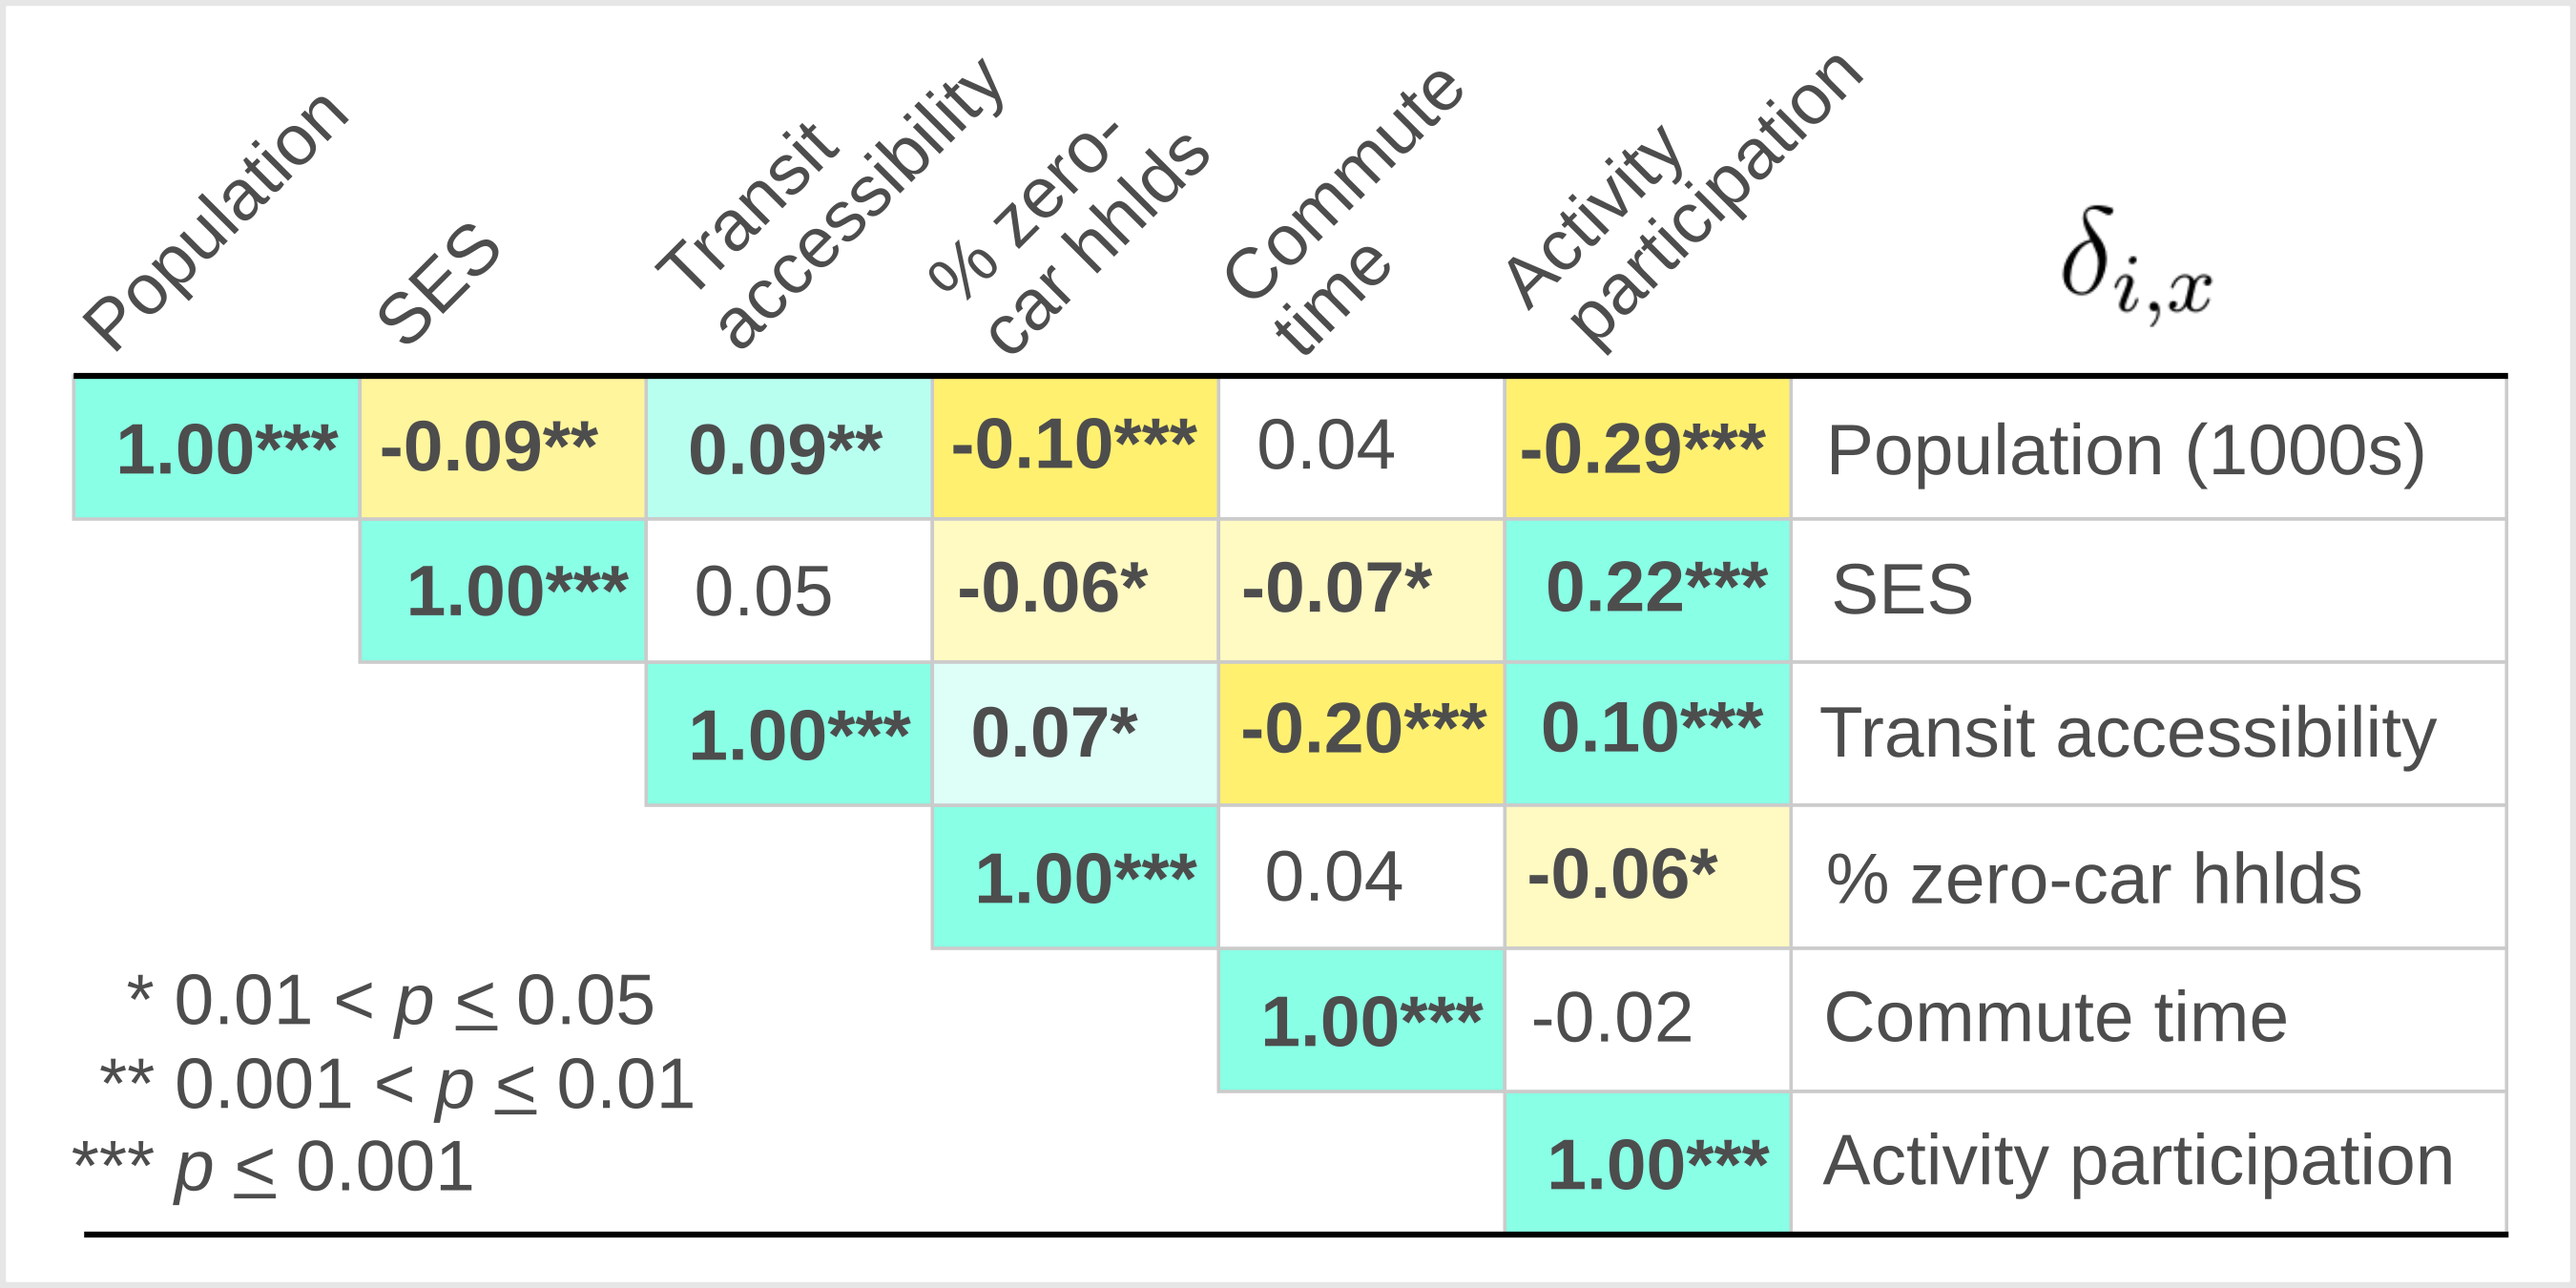
\includegraphics[width=4.5in]{figures/Fig3}
	\caption{{Correlation coefficients between neighborhood change variables}}
	\label{fig:beta_cormod}
\end{figure}


To further explore these relationships, we generate two models to examine the multivariate effects of social and transport disadvantage on adverse travel behaviour outcomes: increasing commute times and declining activity participation rates. These are modelled as follows.

\begin{equation}
Y = \rho W Y + \Theta X + \epsilon
\end{equation}

Where $Y$ is the vector of dependent variables (change in neighborhood averages of commute times and activity participation rates, respectively), $X$ is a matrix of independent variables, $\Theta$ is a vector of coefficients, and $\epsilon$ are the error terms. The models were originally specified using ordinary least squares regression, but we found significant positive spatial auto-correlation among the residuals, leading to specifying a model that incorporates spatial effects \cite{anselin_spatial_1988}. A Lagrange multiplier test was used to decide on using a spatial lag model rather than a spatial error model \cite{anselin_exploring_2005}. This is incorporated via a spatial auto-regressive component, $\rho W Y$, where $\rho$ is a spatial lag parameter and $W$ is a row normalized Queen connectivity spatial weights matrix. Results are displayed in Table \ref{table:model}. In addition to the variables included in the map in Figure \ref{fig:change_maps}, we also included an independent variable representing change in the percent elderly population in each neighborhood since previous research has noted that the elderly travel less than the non-elderly population \shortcite{newbold_travel_2005,xu_good_2018}.


\begin{table}[h]
	\small
	
	\caption{{Model results showing how neighborhood change in social and transport disadvantage effects changes in travel behaviour}}
	\label{table:model}
	\begin{adjustwidth}{-1in}{-1in}
		
		\centering
	\begin{tabular}{lcccc}
		\hline
		& \multicolumn{2}{c}{\textbf{Change in activity participation}} & \multicolumn{2}{c}{\textbf{Change in commute time}} \\
		\hline
		n                & \multicolumn{2}{c}{1133}      & \multicolumn{2}{c}{1133}       \\
		pseudo-R2               & \multicolumn{2}{c}{0.26}      & \multicolumn{2}{c}{0.16}       \\
		\hline
		& \textbf{Coefficient}      & \textbf{\textit{p}-value}         & \textbf{Coefficient}     & \textbf{\textit{p}-value}         \\
		\hline
		$\alpha$ & -0.004           & 0.000     & 0.145           & 0.000     \\
		$\rho$      & 0.400            & 0.000     & 0.388           & 0.000     \\
		Change in population (1000s)      & -0.019           & 0.000     & 0.091           & 0.142     \\
		Change in $SES_i$      & 0.019            & 0.000     & -0.159          & 0.235     \\
		Change in $A_{i,\lambda}$       & 0.281            & 0.003     & -16.250         & 0.000     \\
		Change in \% zero-car households   & -0.002           & 0.002     & 0.044           & 0.013     \\
		Change in \% elderly (65+)  & -0.003           & 0.003     & -0.111         & 0.000    \\
		\hline
	\end{tabular}

	\end{adjustwidth}
\end{table}

The commute time model indicates that increases in transit accessibility and car ownership are linked to reduced commute times, indicating a strong relation to transport disadvantage, overall. Change in SES over time, however, is not found to have a significant association with changing commute times, after controlling for other variables. 


For the activity participation models, we find that growing social and transport disadvantages are both related to declining participation rates. This shows that the fewer resources people have, transport and socio-economic, the less likely they are able to travel to and participate in daily activities. This corroborates previous theoretical and cross-sectional findings on how social and transport disadvantage limit the ability to travel and participate in daily activities, a key indicator of transport poverty \cite{roorda_trip_2010,lucas_transport_2012,lucas_is_2018,allen_planning_2020}. The findings in Table \ref{table:model} show that these trends are also true when examining changes in transport and social disadvantage over time, and lend a somewhat more causal explanation to the observed changes.




\subsection{Suburbanization of Transport Poverty}

In this section, we further examine whether neighborhoods with increasing social and transport disadvantage are occurring more in suburban areas compared to central neighborhoods. To do so, we first need to consider what counts as "suburban". Previous research has used metrics like distance to the urban centre, age of housing stock, and population or housing density, and often result in binary definitions of city versus suburb to describe how centralized or suburbanized a neighborhood is \cite{massey_dimensions_1988,cooke_suburbanization_2015}. Instead, we use our transit accessibility measure to quantify suburbanization, as it is a combination of land-use patterns and connectivity. Transit accessibility is also a predictor of auto-ownership \cite<e.g.>{klein_millennials_2017} and can thus be used to explain how auto-dependent a neighborhood is. Specifically, we take $A_{i,\lambda}$ and average it over the 1991 to 2016 period, $\bar{A}_{i,\lambda}$, as a proxy for neighborhood-level suburbanization. 

We then plot how changes in social and transport disadvantage are related to this accessibility-based level of suburbanization. This is displayed in Figure \ref{fig:sub_pov}. The Y-axes on these plots are values of rates of change from 1991 to 2016 for different variables computed in the previous section. The X-axes are $\bar{A}_{i,\lambda}$ and the legend on the bottom of this figure approximately describes the type of urban form that is associated with different ranges of accessibility. Each dot represents a neighborhood and the curves displayed were fitted via a generalized additive model based on regression splines \cite{wood_smoothing_2016}. The curves describe a moving-window average of how each variable has changed over time for different levels accessibility.

\begin{figure}[H]
	\centering
	\vspace{2mm}
	\hspace*{-0.333in}
	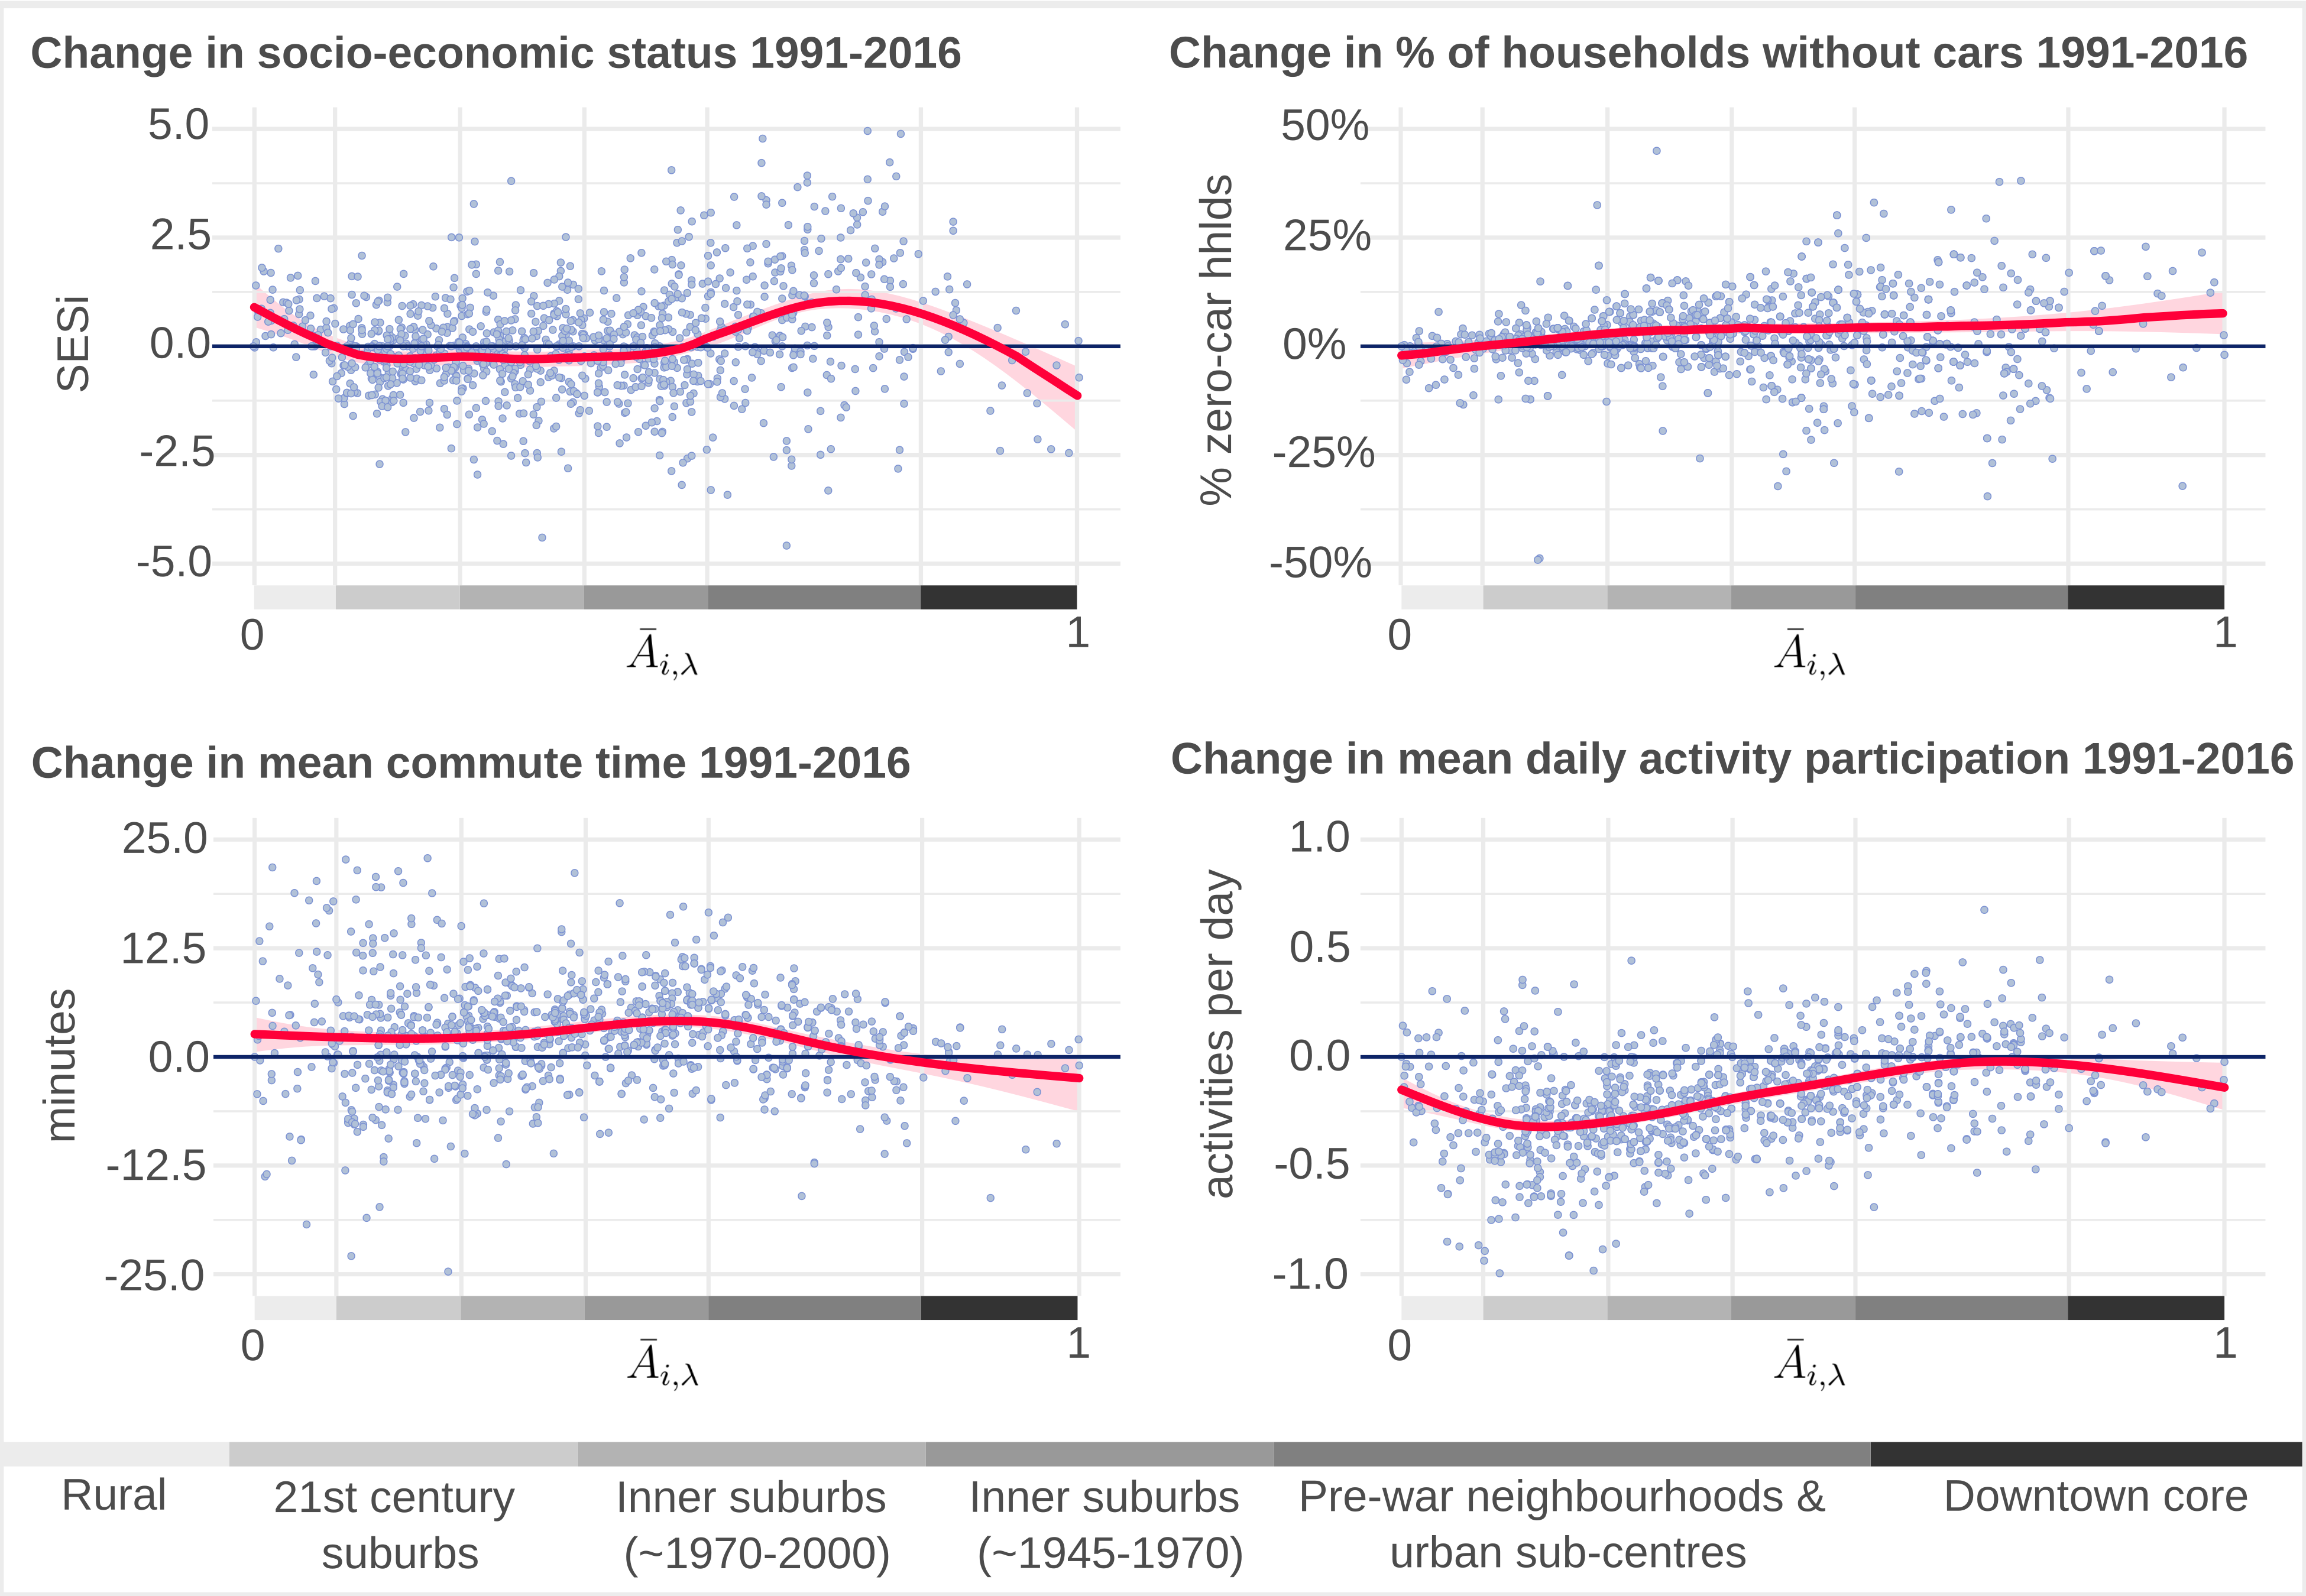
\includegraphics[width=6.5in]{figures/Fig4_sub_plot_4.png}
	\caption{{Change in SES, car ownership, and travel behaviour in Toronto by an accessibility-defined measure of urban form}}
	\label{fig:sub_pov}
\end{figure}

The top-left of this figure shows change in SES by neighborhood. We find that pre-war neighborhoods have substantially improved in terms of SES and that suburban neighborhoods have on average slightly declined in terms of SES. This confirms previous research that has highlighted trends of gentrification occurring close to the core and a decline or stagnation in SES in many suburban neighborhoods \cite{ades_are_2012,hulchanski_three_2010,walks_social_2001,ades_is_2016}. The top-right shows that zero-car households have increased relatively evenly throughout the spectrum of urban structure, with the greatest increase occurring in the downtown core, where there are the highest levels of transit accessibility. The downtown core has also experienced the greatest increase in housing costs over this 25 year period.

Looking at the bottom two plots on changes in travel outcomes over time, we find that commute times have increased more within suburban areas, with a small bump particularly within the inner-suburbs. Only central neighborhoods have witnessed a reduction in commute times on average. Activity participation rates have declined overall, but we observe that this decline is occurring predominantly in suburban neighborhoods. Suburban areas are thus experiencing the brunt of increasing adverse travel behaviour outcomes in the region.

Transport poverty has been described as the compounding of both social and transport disadvantage \cite{lucas_transport_2012, lucas_is_2018}. Accordingly, for our last piece of analysis, we generate a composite measure for examining the extent to which neighborhoods are increasing or decreasing signs of experiencing transport poverty, $\delta_{TP,i}$, and then visualize it's spatial distribution. In particular, we are interested in whether transport poverty is increasing more within the suburbs than central neighborhoods. To generate $\delta_{TP,i}$, we sum the standard scores of $\delta_{i,x}$ for five pertinent variables $x$: change in socio-economic status ($SES_i$), transit accessibility ($A_i$), percent zero-car households, mean commute times, and mean daily activity participation rates. 

\begin{equation}
\delta_{TP,i} = \sum_x \frac{\delta_{x,i} - \mu_{\delta_{x}}}{\sigma_{\delta_{x}}}
\end{equation}

The signs of each $\delta_{i,x}$ are set that positive values of $\delta_{TP,i}$ can be interpreted as neighborhoods with increased travel barriers and worse travel behaviour outcomes over time. Conversely, negative values of $\delta_{TP,i}$ can be interpreted as neighborhoods where signs of transport poverty are decreasing over time, on average. Figure \ref{fig:tpov} visualizes the spatial distribution of $\delta_{TP,i}$ (right) as well as plots $\delta_{TP,i}$ relative to mean levels of transit accessibility $\bar{A}_{i,\lambda}$ (left).

We observe that transport poverty is decreasing substantially in older, centrally located, neighborhoods; gentrifying neighborhoods with salutary levels of transit accessibility and walkable built environments. Conversely, more auto-oriented suburban neighborhoods, on average, are witnessing increases in risks of transport poverty over time. There is, however, quite a bit of variation across this spectrum of urban form. The orange and red areas on the map are those in which transport poverty has increased substantially from 1991 to 2016. Clearly this has occurred in inner-suburban neighborhoods in the east (primarily in Scarborough), as well as more distant suburban areas to the east, north, and northwest. However, this is not to say that all suburbs follow this trend, there are still a number of suburban neighborhoods showing signs that transport poverty is declining over time. These tend to be a combination of neighborhoods where SES has not declined and neighborhoods where transit accessibility has improved. This is particularly evident in the western suburban areas that have witnessed improvements in transit accessibility. Overall, the key finding here is that risks of transport poverty are increasing more within auto-oriented suburban areas than compared to centrally located neighborhoods. 


\begin{figure}[H]
	
	\centering
	
	
	\hspace*{-0.333in}
	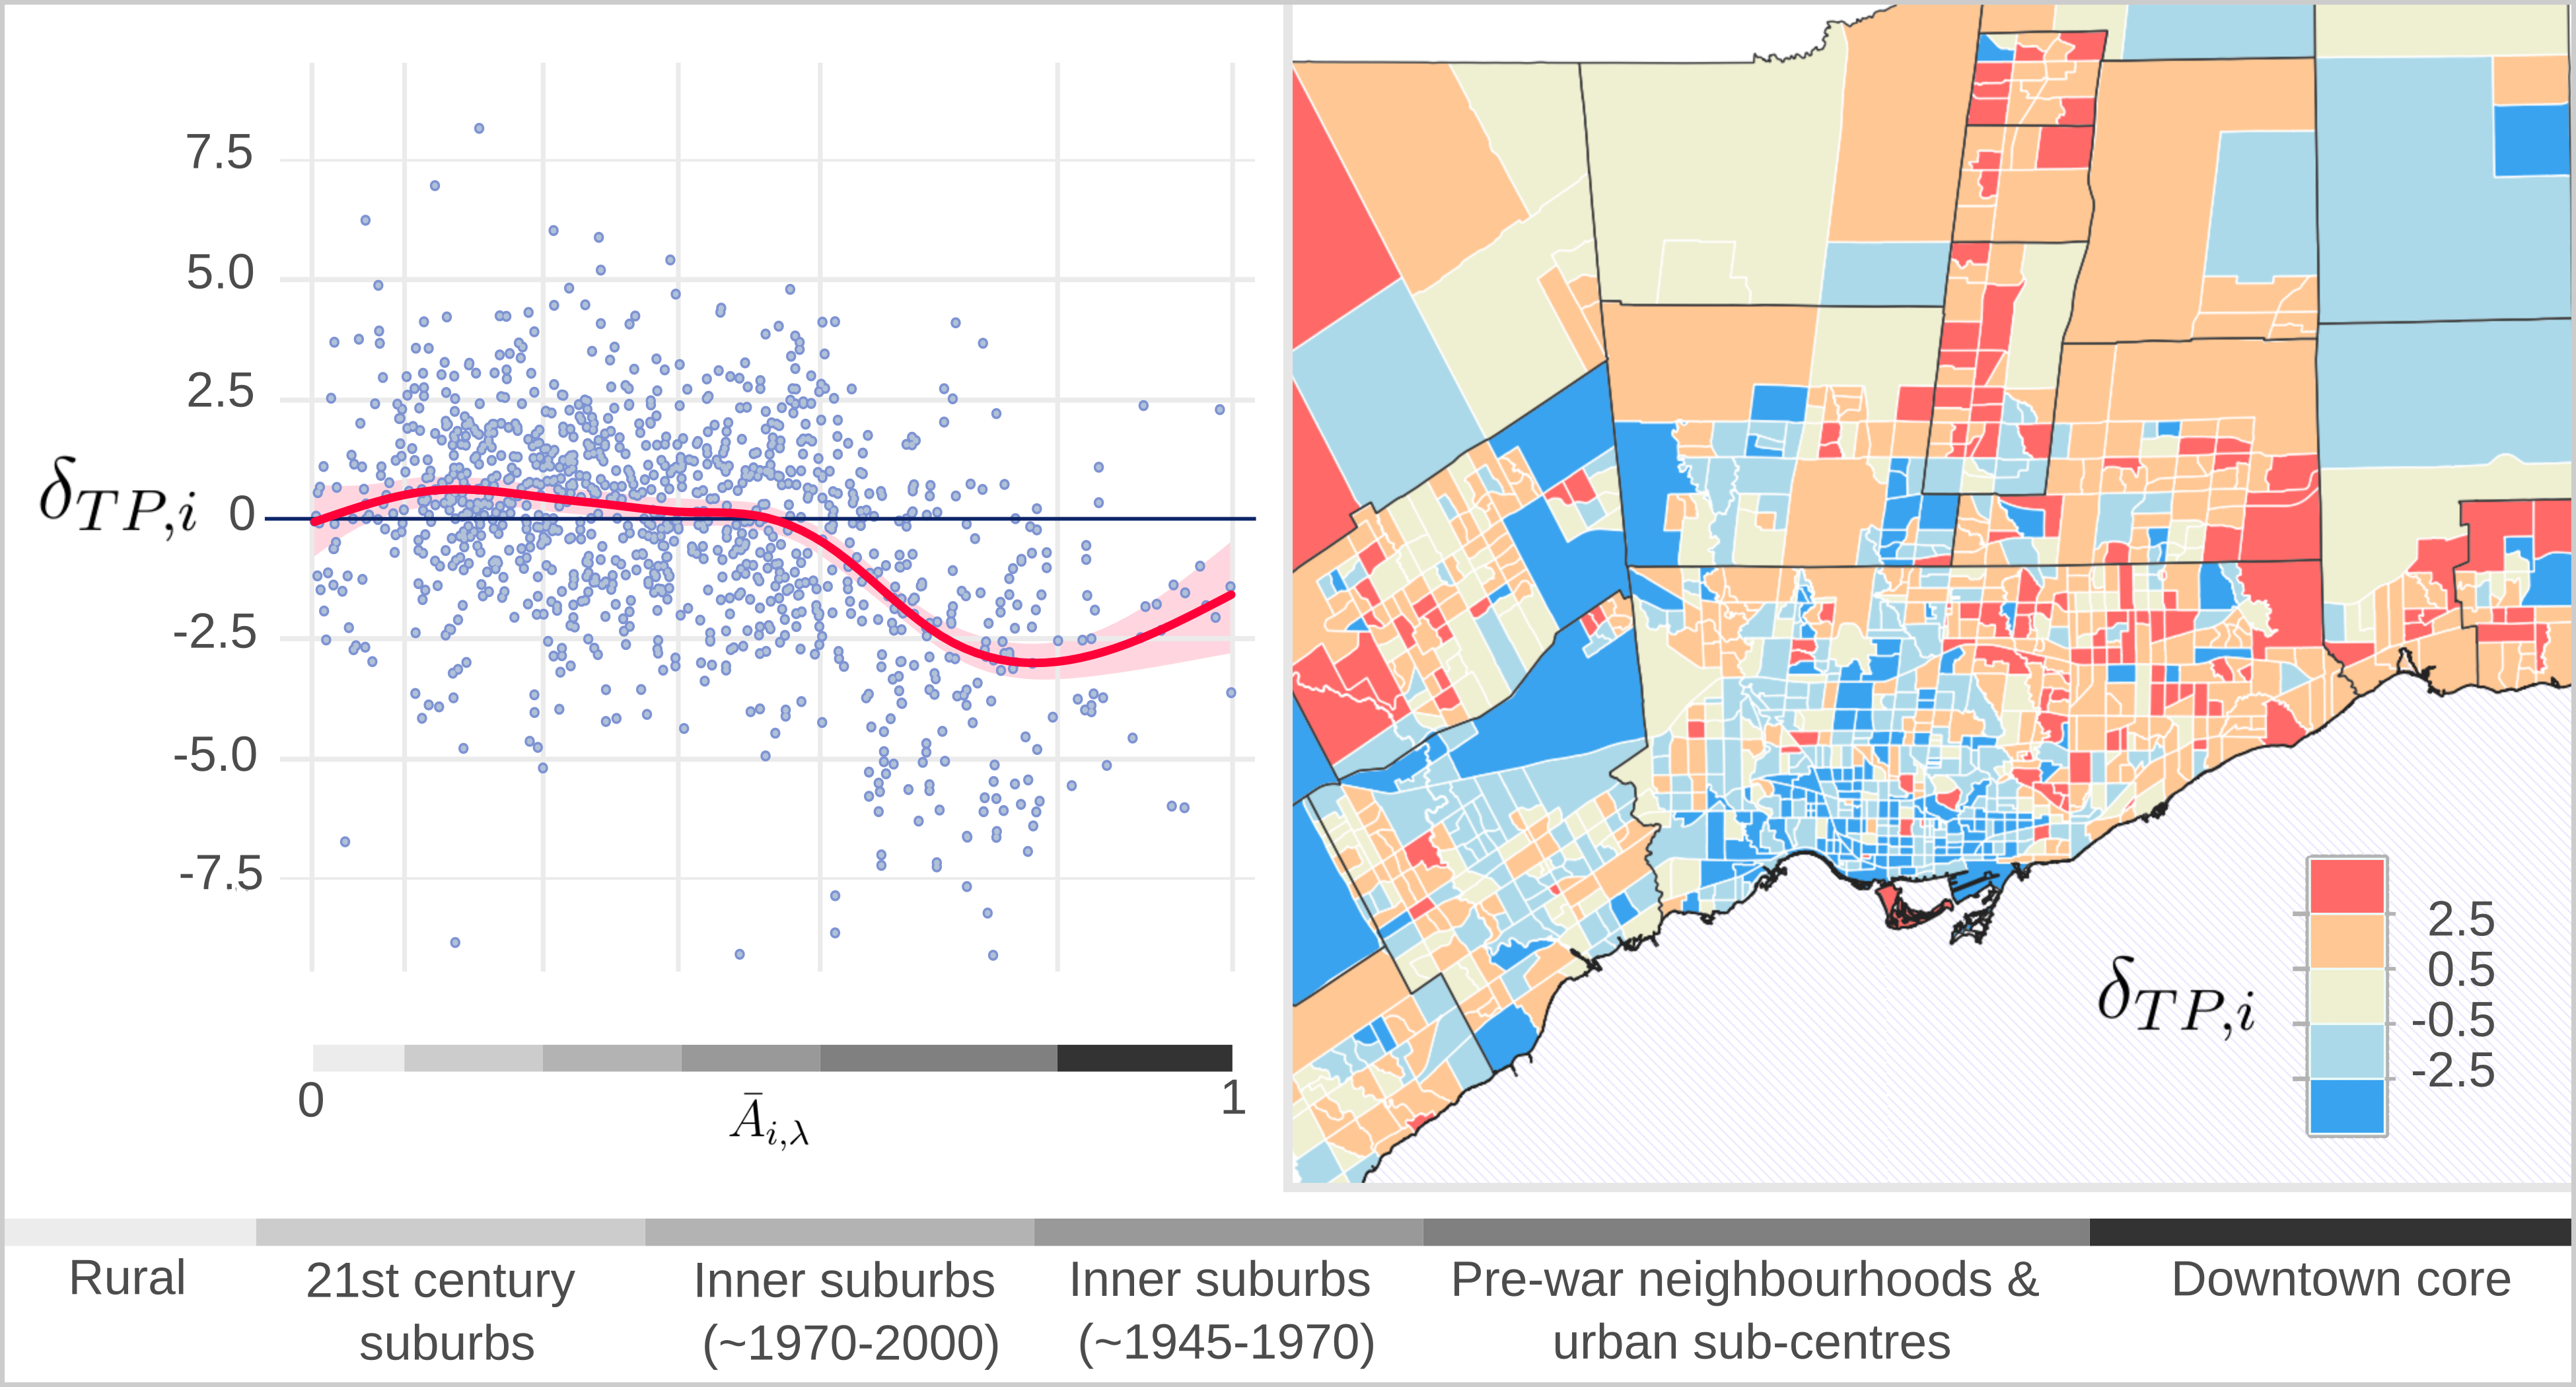
\includegraphics[width=6.5in]{figures/Fig5_tp_time.png}
	
	
	\caption{{Change in transport poverty, $\delta_{TP,i}$, by mean level of accessibility (left). Map of change in $\delta_{TP,i}$ (right).}}
	\label{fig:tpov}
\end{figure}



\section{Conclusions}

% limitations
Our study was not immune to limitations, and thus offers directions for future work. For one, our research focused on transport (dis)advantage in terms of transit access to destinations and auto ownership, but we did not consider other components of urban form that could either benefit or detriment urban living. For example, despite gains in transit access, suburban built environments typically remain focused on the car, which have a number of safety and environmental concerns (e.g. speed limits are greater, safe crossings are more spread out, creating barriers to active travel). On the other hand, some suburban areas offer better access to green space, which can have a positive effect on health and well-being. Future research should consider other positive and negative environmental impacts of less-centralized urban living for low-SES populations. This could prove challenging, however, since there is little readily available historic data on urban form, walkability, and access to green space.

Our study also had some other data limitations. We relied on a travel survey that represented a 5\% sample of the population, limiting analysis at smaller geographic scales. Secondly, there may have been some inconsistencies with how data were collected across survey years. We did select variables that were consistently defined over time based on survey documentation, but there were likely some imperfections in interpretation and administration of survey questions. As well, in terms of data, there was likely some inaccuracy caused by the data harmonization process of apportioning data to the same spatial units. These issues are unavoidable when dealing with longitudinal survey data that has been aggregated to different areal units \cite{allen_new_2018}. 

As well, our neighbourhood-level analysis could be masking individual effects since we only analyzed change at a neighborhood level. For example, there could be more extreme levels of travel be outcomes in later years than earlier years in certain neighborhoods. However, the data are limited in that specific individuals are not tracked over time, preventing the possibility of a true individual-level panel study. These problems highlight the need in the future for individual-level linked datasets, similarly to how medical records have been linked to census data in health research. Analyzing individual panel data would be helpful for examining pathways to suburban poverty and whether improvements in transit accessibility are either more likely to alleviate poverty or result in gentrification and displacement.

Despite these limitations and important directions for future work, our study provides solid evidence that transport poverty in Toronto is increasing more in the suburbs relative to central areas. Eastern suburbs in particular have suffered the most, indicative by having the greatest combination of increased transport and social disadvantage, and evidenced by increasing commute times and declining daily activity participation rates. Our research thus confirms theoretical pathways of transport poverty \cite{lucas_transport_2012}, and moreover, shows that it is occurring more within suburban neighborhoods.

Policy to reduce these effects should thus have a two-pronged approach. The first is to curb the growth of suburban poverty through focusing on increasing the supply of affordable housing in areas with high transit accessibility, having strong rent controls, and preventing forced eviction and displacement from central to suburban neighborhoods. The second is to upgrade suburban environments through transport planning and urban design strategies that improve transit accessibility and walkability (i.e. improving accessibility at both neighborhood and regional scales). These are not new ideas. Many of them have been advocated for previously in terms of reducing the negative population health and environmental impacts associated with auto-oriented environments \shortcite{cervero_travel_1997,ewing_relationship_2003,ewing_compactness_2015}, and limiting the detrimental impacts suburbanization of poverty has on increasing polarization and segregation of urban space as well as the negative impacts caused by eviction and displacement on individual well-being and community cohesion  \shortcite{hulchanski_three_2010,ades_are_2012,walks_income_2013,august_challenging_2014,august_its_2016}. Our research provides one more important piece of evidence showing that such strategies would also be progressive options in reducing barriers to daily travel and transport-related social exclusion.








\section*{3.A \hspace{1mm} Appendix}
\addcontentsline{toc}{section}{3.A \hspace{1mm} Appendix}

\subsection*{3.A.1 \hspace{2mm} Selection of distance decay parameters for measuring accessibility}
\addcontentsline{toc}{subsection}{3.A.1 \hspace{2mm} Selection of distance decay parameters for measuring accessibility}


For our accessibility measures, we used a negative exponential impedance function in order to weight nearby destinations more than those further away (see Section 3.3). This was defined as follows:

\[f(t_{i,j}) = e^{\beta t_{i,j}}\]

Where $t_{i,j}$ is the travel time and $\beta$ is a decay parameter. As we noted in the main text, we followed the advice by \citeA{osth_new_2016} that $\beta$ can be approximated by selecting the curve which returns 0.5 for the median travel time. This is based on their argument that such a selection can adequately approximate origin-destination trip flows in spatial interaction modelling as well as for its ease of interpretation \cite{osth_new_2016}. This led to the selection of $\beta = -0.0277$ for access to jobs and $\beta = -0.0462$ for access to non-work destinations

To further assess the validity of this selection of $\beta$, we first looked at previous research which has measured accessibility over multiple time periods in the Toronto region. There are four studies that we are aware of. The first, by \citeA{foth_towards_2013} claims to use a gravity-based formulation to measure access to jobs. Unfortunately, they do not describe how this function is defined. Two papers, one by \citeA{farber_transit_2017} and the other by \citeA{deboosere_understanding_2019} use cumulative measures of accessibility in their analysis. Cumulative measures are less theoretically sound than those which use continuous decay functions as they over-simplify what is accessible by use of a single isochrone. Most applicable to our study is a recent paper \citeA{kasraian_multi-decade_2020} who select a $\beta$ value of -0.05 when measuring access to population in the Greater Toronto and Hamilton Area. \citeA{kasraian_multi-decade_2020} derive this value of $\beta$ from another rule of thumb \cite{batty_proximate_1984}, where $\beta$ is equal to one divided by the mean travel time (20 minutes was the mean travel time for all trips selected for use in their study). They also justify their selection based on that "travel time parameters in operational travel demand models for the region have consistently fallen within the 0.02–0.06" range \cite{kasraian_multi-decade_2020}. For our study, initially based on the advice from \citeA{osth_new_2016} we used a $\beta$ value of -0.0277 for access to jobs and -0.0462 for access to non-work destinations. These both fall within this -0.02 to -0.06 range. Moreover, if we followed the 
\citeA{batty_proximate_1984} approximation used by \citeA{kasraian_multi-decade_2020}, our values of $\beta$ would be -0.0316 (difference of 0.0039) for access to jobs, an -0.0505 (difference of 0.0043) for access to non-work destinations. These are very close to our selected values.

For the sake of sensitivity, we computed access to jobs using $\beta$ values of 0.02, 0.03, 0.04, 0.05, and 0.06 to show the similarity in results across this range. Below is a correlation matrix of the resulting accessibility measures.

\begin{table}[h]
	\vspace{2mm}
	\small
	\centering
	\caption{Correlation among measures of access to jobs by transit for different values of $\beta$}
	\label{table:beta_cor}
	\begin{tabular}{llllll}
		\hline 
		$\beta$  & -0.02 & -0.03 & -0.04 & -0.05 & -0.06 \\
		\hline
		-0.02 & 1.000 & 0.985 & 0.950 & 0.903 & 0.850 \\
		-0.03 &       & 1.000 & 0.989 & 0.960 & 0.921 \\
		-0.04 &       &       & 1.000 & 0.991 & 0.967 \\
		-0.05 &       &       &       & 1.000 & 0.993 \\
		-0.06 &       &       &       &       & 1.000   \\ \hline 
	\end{tabular}
\end{table}

Clearly there is quite high correlation among these measures, and selecting any value within this range (-0.02 to -0.06) would likely have only very minor differences in results, particularly since we were primarily concerned with relative changes in accessibility over time, rather than absolute values at a particular point in time. 

Furthermore, we also fitted negative exponential curves based on the distribution of trips by their travel times (at minute-by-minute intervals). We did this for the two types of trip purposes and subsequent accessibility measures that we generated, for home-to-work trips ($\beta_W$), and for trips to non-work activity destinations ($\beta_{NW}$). The resulting values are shown below.

\begin{table}[h]
	\vspace{2mm}
	\small
	\centering
	\caption{Values of $\beta$ fitted from travel survey data for Toronto}
	\label{table:beta_fit}
	\begin{tabular}{lll}
		\hline
		Year & $\beta_{W}$ & $\beta_{NW}$ \\ \hline
		1991 & -0.0269   & -0.0389       \\
		1996 & -0.0255   & -0.0464       \\
		2001 & -0.0272   & -0.0399       \\
		2006 & -0.0325   & -0.0426       \\
		2011 & -0.0312   & -0.0521       \\
		2016 & -0.0279   & -0.0486       \\
		All$^*$  & -0.0289   & -0.0432      \\ \hline \\
	\end{tabular}
	
	$^*$All years combined before fitting
\end{table}

We find that each of these values is within a range of less than 0.01 of the $\beta$ values used in our analysis. Extrapolating from our correlation noted above, it is unlikely that selecting one of these fitted $\beta$ values will result in an accessibility measure that is substantially different from what we used. In fact, when looking at the correlations between accessibility measures only 0.01 apart, they are all above 0.98.

To conclude, we believe our selection of $\beta$ is appropriate for our analysis given precedent in the literature, fitted values from data, correlation between accessibility measures, and comparing with the range of values that have been used in previous studies (-0.02 to -0.06). 

Overall, the goal of our study was focused more on the application of accessibility alongside several other socio-economic and transport-related variables to study suburbanization of poverty, rather than specifically and solely focused on developing accessibility measures. Nevertheless, we do think that more work could be done in the future to derive more accurate accessibility measures that are suitable for longitudinal analyses. Clearly our paper, and some of the other papers that we cited above, would benefit from such work to move beyond these relatively simplistic approximations. Doing so would require additional thought about how to appropriately work with matrices from multiple time periods, multiple travel modes, changes in infrastructure, and different sample sizes when fitting spatial interaction models.

